\documentclass[letter]{article}
\usepackage[]{float}
\usepackage[monocolor]{../math232/ahsansabit}

\title{Heat Light and Waves : : Homework 08}
\author{Ahmed Saad Sabit, Rice University}
\date{\today}

\begin{document}
\maketitle
\section*{Problem 01}
\subsection*{(a)} 
\begin{align*}
	v_1 &= \frac{c}{n_1} \\
	v_2 &= \frac{c}{n_2} 
\end{align*} 
\begin{align*}
	d_1 &= \sqrt{h_1^2 + x^2}  \\
	d_2 &= \sqrt{h_2^2 + (L - x)^2}  \\
\end{align*}
\[
\boxed{
t = n_1 
\frac{\sqrt{h_1^2 + x^2} }{c} + 
n_2 
\frac{\sqrt{h_1^2 + (L - x)^2 } }{c}
}
\] 

\subsection*{(b)} 
\begin{align*}
	\frac{\mathrm{d} t}{\mathrm{d} x} = 0 &= \frac{n_1}{c} 
	\frac{x}{\sqrt{h_1^2 + x^2 }  } -
	\frac{n_2}{c} \frac{L-x}{\sqrt{h_1^2 + (L - x)^2 } } 
	\\
					      &\implies
					      n_1 
					      \left(\frac{x}{\sqrt{h_1^2 + x^2} }\right) 
					      =
					      n_2 
					      \left(\frac{L - x}{\sqrt{h_1^2 + (L - x)^2} }\right) \\ 
					      &\implies
					      n_1 \sin \theta_1 = n_2 \sin \theta_2 
\end{align*}



\section*{Problem 02} 
\subsection*{(a)} 
Look at critical angles first. 
\[
\sin \theta_C = \frac{n_2}{n_3}
\]
Now using that related to $\theta_m$
\begin{align*}
n_1 \sin \theta_m &= n_3 \sin \theta_2 \\
\sin \theta_m &= n_3 \cos \theta_c \tag{$90^{\circ} - \theta_{2,m} = \theta_c $} \\ 
\theta_m &= \arcsin \left(n_3 \sqrt{ 1 - \left(\frac{n_2}{n_3} \right)^2} \right) \\
\end{align*}
Hence what we get is 
\[\boxed{
\theta_m = \arcsin \left(\sqrt{n_3^2 - n_2^2} \right)
}\]
Similar problem : Asian Physics Olympiad 2024 Theory Examination. 



\subsection*{(b)} 
Writing the obvious equations and finding them using the calculator
\begin{align*}
	n_3 \sin \theta_\text{core} &= n_2 \implies \text{numerically, } \theta_\text{core} = 59.97^{\circ} \\
	n_2 \sin \theta_\text{clad} &= n_1 \implies \text{numerically, } \theta_\text{clad} =50.27^{\circ}	 
\end{align*}
\begin{align*}
	n_3 \sin \theta_3 &= n_2 \sin \theta_\text{clad} \\ 
			  &\implies \text{numerically, } \theta_3 = \arcsin 
			  \left(\frac{n_2}{n_3} \sin \theta_\text{clad}\right) = 41.81 ^{\circ}
\end{align*}
which satisfies $\theta_3 < 59.97^{\circ}$

\subsection*{(c)} 
\[
\cos \theta_2 = \cos \left(90 ^{\circ} - \theta_\text{core}\right) = \sin \theta_\text{core} = \frac{n_2}{n_3}
\] 
\[
t_1 = \frac{L}{c / n_3} = \frac{L n_3}{c}
\] 
\[
t_2 = \left(L / \cos \theta_2\right) / (c / n_3) = \frac{L n_3^2 }{c n_2}
\]
\[
\Delta t = t_2 - t_1 = \frac{L n_3^2}{c n_2} - L \frac{n_3}{c} = \frac{L n_3}{c} \left(\frac{n_3}{n_2} - 1\right)
\] 
\[
\boxed{
\Delta t = n_3 \left(\frac{n_3}{n_2} - 1\right) \frac{L}{c}
}
\] 
\section*{Problem 03}



\subsection*{(a)} 
\begin{align*}
	\frac{1}{f_2} &= \frac{1}{d} + \frac{1}{x} \\ 
	\frac{2}{R_2} - \frac{1}{d} &= \frac{1}{x}  \\ 
	\frac{1}{
\frac{2}{R_2} - \frac{1}{1 - 0.75} 
} &= x \implies x =-0.136 \, \text{m}
\end{align*}
\[
\boxed{
D = x- d = 0.886 \, \text{m}
}
\] 

\subsection*{(b)} 
\[
R_1 = 1 \, m
\] 
\[
f_1 = 0.5 \, m
\] 
Leaving $R_2$ as unknown
\[
d = 0.5 \, m - 0.75 \, m
\] 
\[
\frac{1}{f_2} = \frac{1}{-0.25} + \frac{1}{-0.136} \implies f_2 = -0.088 \, m
\] 
\[
R_2 = 2 f_2 = - 0.176 \, m 
\] 
The secondary mirror should be a convex mirror with radius $-0.176 \, m$

\section*{Problem 04} 
\begin{figure}[H]
	\centering
	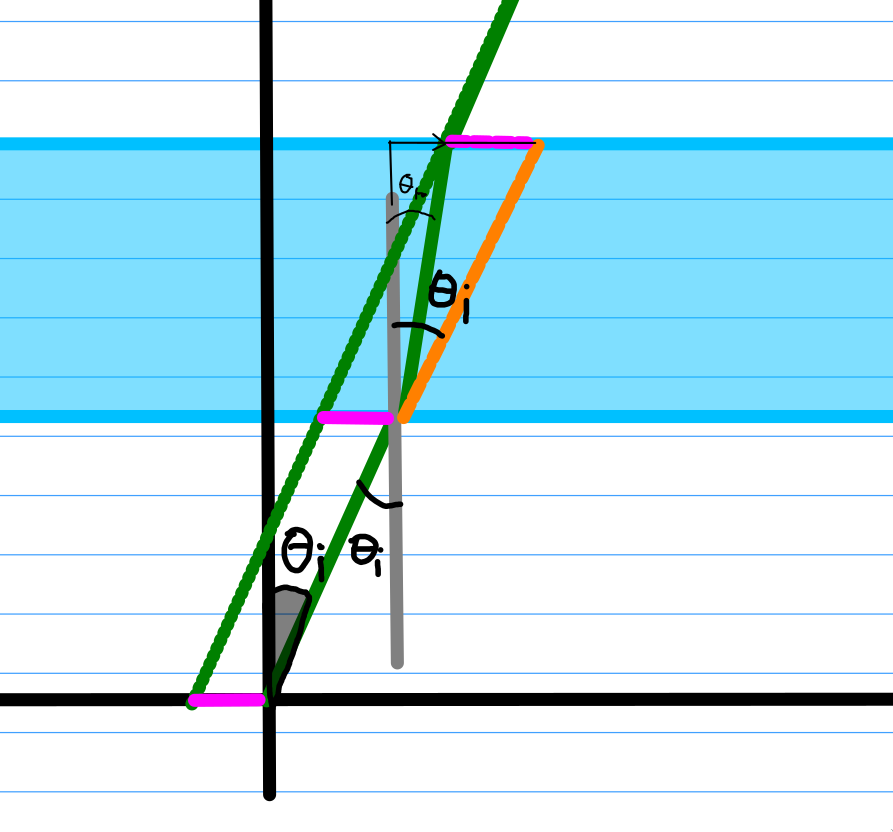
\includegraphics[width=0.8\textwidth]{./ss/8/1.png}
	\caption{./ss/8/1.png}
	\label{fig:-ss-8-1-png}
\end{figure}
We just need to care about the Purple colored line which is the shift of the image. 
With small angle, \[
\sin \Theta_i = n \sin \Theta_r \implies \Theta_r \approx \frac{\Theta_i}{n}
\] 
\begin{align*}
	\Delta x &= (4) (\tan\left(\Theta_i\right)  - \tan \left(\Theta_r\right))\\ 
	&= 4 \left(
\frac{\sin \Theta_i}{\sqrt{1 - \sin ^2 \Theta_i} } -
\frac{\sin \Theta_r}{\sqrt{1 - \sin ^2 \Theta_r} }
\right) \\ &
	\approx 4 
	\left(
\frac{\theta_i}{\sqrt{1 - \theta_i^2} } - 
\frac{\theta_i / n }{\sqrt{1 - \frac{\theta_i^2}{n^2}} }
	\right)
	\\ &
	\approx 4 \theta_i \left(1 - \frac{1}{n}\right) = 1.42 \theta_i
\end{align*}
The shift in the position is a function of the small incident angle $\theta_i$ 


\textbf{NOTE}: Geometrically it's obvious the shift in the image has NO dependence on the distance between the glass from the ground. It's only the angle that matters here.


\section*{Problem 05} 
\subsection*{(a)} 
\begin{align*}
	F &= (n-1) \left(\frac{1}{r_1} - \frac{1}{\infty}\right) \\
	  \implies \frac{F}{n-1} &= \frac{1}{r_1} \implies r_1 = \frac{n-1}{F} = 1.1 \, \text{m}
\end{align*}
\subsection*{(b)} 
\begin{align*}
	n_\text{lens-water} &= \frac{n_\text{lens}}{n_\text{water}} \\
	r_1 &= \frac{ \frac{n_\text{lens} }{ n_\text{water} } - 1}{F} \implies r_1 = 0.33 \, \text{m} \text{ convex when facing it}
\end{align*}


\section*{Problem 06} 
\begin{figure}[H]
	\centering
	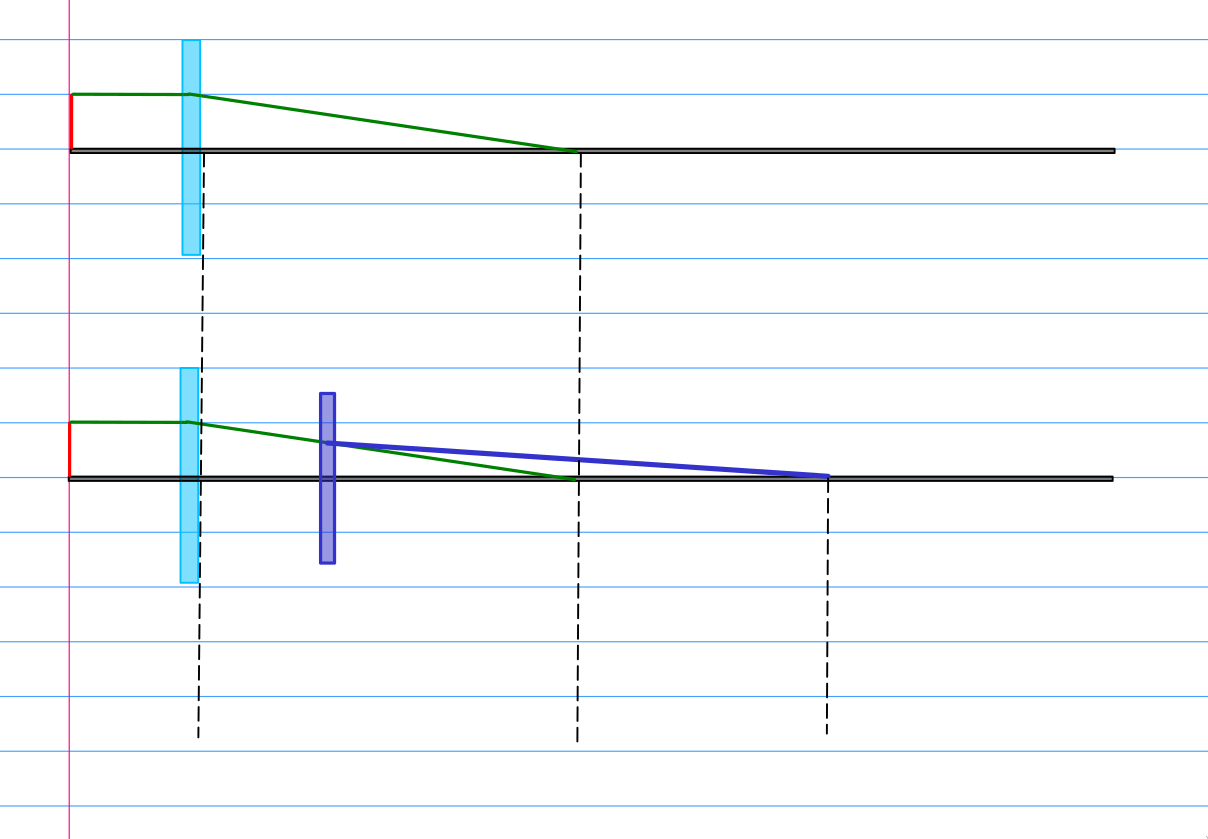
\includegraphics[width=0.8\textwidth]{./ss/8/2.png}
	\caption{./ss/8/2.png}
	\label{fig:-ss-8-2-png}
\end{figure}
\[
\frac{1}{f_2} = \frac{1}{34.2} - \frac{1}{-15} \implies f_2 = 10.43 \, \text{cm}
\] 
\[
\boxed{
f_2 = - 10.43 \, cm
}
\]

\section*{Problem 07} 
\subsection*{(a)} 
\begin{figure}[H]
	\centering
	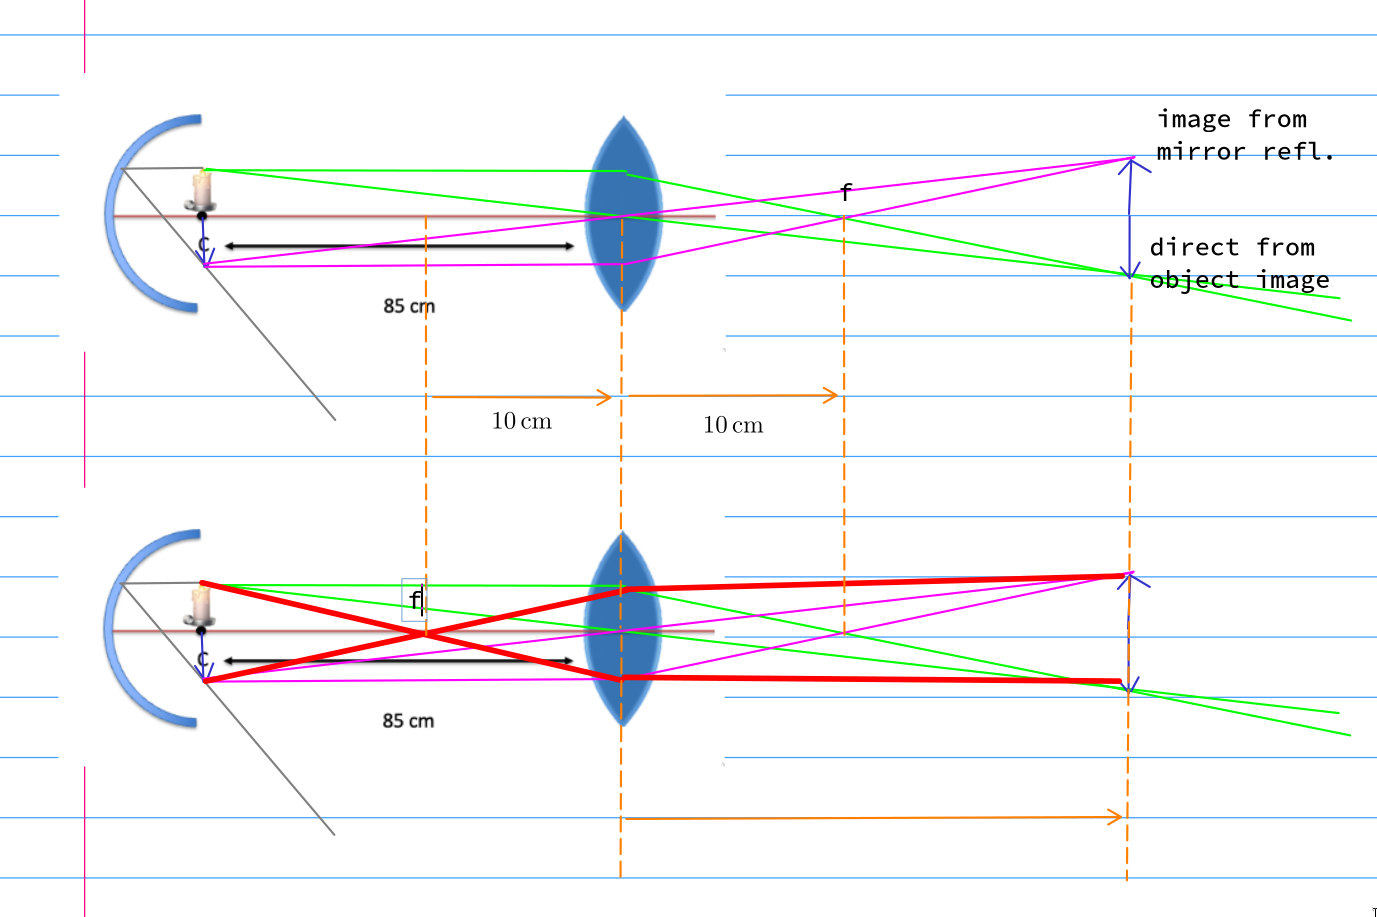
\includegraphics[width=0.8\textwidth]{./ss/8/3.png}
	\caption{./ss/8/3.png}
	\label{fig:-ss-8-3-png}
\end{figure}
\subsection*{(b)} 
For the direct image 
\[
\frac{1}{f} = \frac{1}{x} - \frac{1}{-85} \implies x = 8.95 \, \text{cm}
\]
The image is a real image.
\[
m = - \frac{8.95}{85} = 0.105
\] 
\[
	h' = mh = 0.21 \, \text{cm, upright} 
\] 

For the mirror, 
\[
\frac{1}{10} = \frac{1}{20} + \frac{1}{x} \implies x = 20 \, \text{cm}
\] 
\[
	m_\text{mirror} = - \frac{20}{20} = -1
\]
\[
h' = - 2 \, \text{cm}
\] 
For lens
\[
\frac{1}{10} = \frac{1}{d} + \frac{1}{-85} \implies d = 8.95 \, \text{cm}
\] 
\[
m_\text{lens} = \frac{8.95}{-85} = 0.105 
\] 
\[
h' = - 0.21 \, \text{cm}
\] 
\[
m_\text{total} = -0.1053 \, \text{inverted}
\] 
\end{document}
